\documentclass[12pt]{article}

% --------------------
% Packages
% --------------------
\usepackage[margin=1in]{geometry}
\usepackage{setspace}
\usepackage{graphicx}
\usepackage{hyperref}
\usepackage{pgfplots}
\usepackage{tikz}
\usepackage{float}
\pgfplotsset{compat=1.18}

% --------------------
% Document Info
% --------------------
\title{\textbf{A Strategic Analysis of the TFT Composition: Ekko Reroll}}
\author{Boice Wong}
\date{\today}


% --------------------
% Begin Document
% --------------------
\begin{document}

\begin{titlepage}
  \centering
  \vspace*{\fill}

  {\LARGE\bfseries A Strategic Analysis of the TFT Composition: Ekko Reroll\par}
  \vspace{1.5cm}

  {\large Boice Wong\par}
  \vspace{0.5cm}

  {\large \today\par}

  \vspace*{\fill}
\end{titlepage}

\onehalfspacing

% --------------------
\section{Introduction}
% Provide an overview of the Ekko Reroll composition.
% Discuss why the comp is relevant in the current TFT meta.
% Briefly outline what each section of the thesis will cover. 
\begin{enumerate}
    \item Set 16 is the most flexible TFT set so the obvious playstyle is to hard force a comp. Ekko Chogath Reroll sneaks through the cracks as the ultimate anti-meta hardforce comp.
    \item DISCLAIMER: This comp is a Top 3/4 comp and nowhere near broken... however with the right scenarios, it can win out games completely.
    \item When should you play it? Anytime since it will always be uncontested and people think its bad. The only time you can't hard force this comp is in the triple emblem universe.
	\begin{figure}[h]
	      \centering
	      \includegraphics[width=0.8\linewidth]{photos/ekkoplayrate.png}
	      \caption{Ekko Play Rate (Plat+) Patch 16.1c}
	\end{figure}
    \item The strength in playability of this comp is because in the early game, you play strong board and build items that fit the meta. Unlike other reroll comps, this allows you to enter the line in an infinite amount of ways. In general, the items are extremely flexible and supportive of slamming for tempo. Nearly every component is good in this comp.

\begin{figure}[H]
\centering
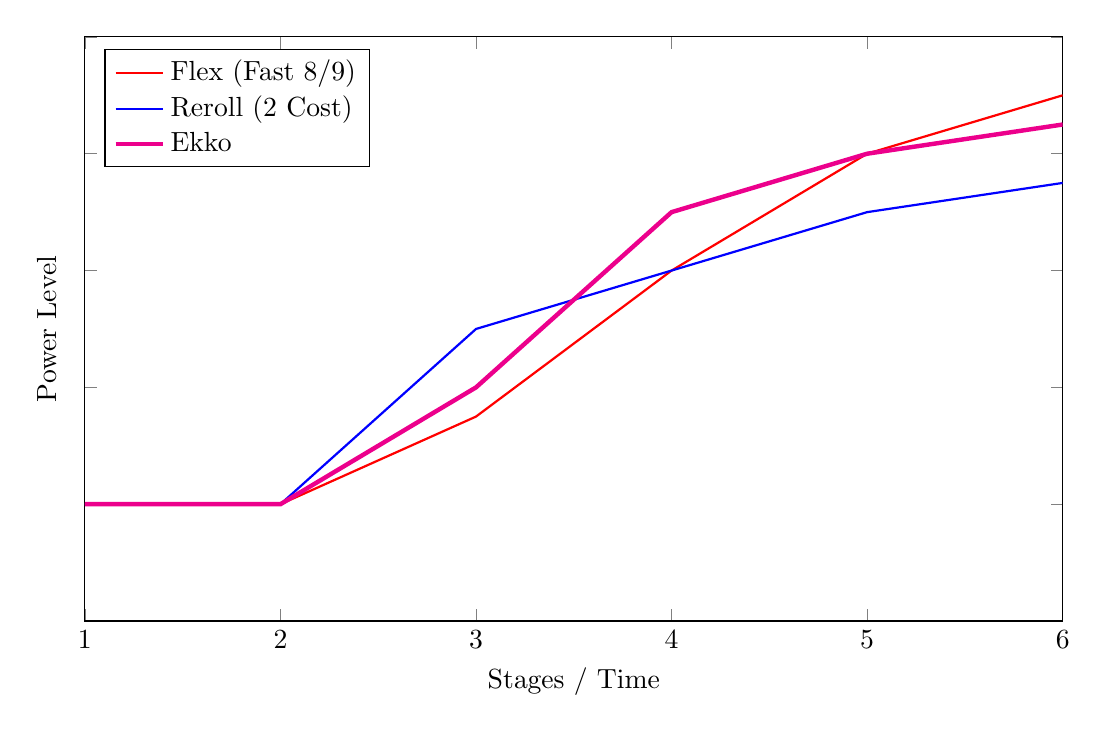
\begin{tikzpicture}
\begin{axis}[
    width=14cm,
    height=9cm,
    xlabel={Stages / Time},
    ylabel={Power Level},
    xmin=1, xmax=6,
    xtick={1,2,3,4,5,6},
    ymin=0, ymax=100,
    yticklabels=\empty
    grid=both,
    legend style={at={(0.02,0.98)},anchor=north west},
    legend cell align=left
]

% --------------------
% FLEX (RED)
% --------------------
\addplot[
    red,
    thick,
    mark=circle
]
coordinates {
    (1,20)
    (2,20)
    (3,35)
    (4,60)
    (5,80)
    (6,90)
};
\addlegendentry{Flex (Fast 8/9)}

% --------------------
% REROLL (BLUE)
% --------------------
\addplot[
    blue,
    thick,
    mark=none
]
coordinates {
    (1,20)
    (2,20)
    (3,50)
    (4,60)
    (5,70)
    (6,75)
};
\addlegendentry{Reroll (2 Cost)}

% --------------------
% EKKO (PINK / MAGENTA)
% --------------------
\addplot[
    magenta,
    ultra thick,
    mark=none
]
coordinates {
    (1,20)
    (2,20)
    (3,40)
    (4,70)
    (5,80)
    (6,85)
};
\addlegendentry{Ekko}

\end{axis}
\end{tikzpicture}
\caption{Relative Power Curves Across TFT Game Stages}
\end{figure}



\end{enumerate}

% --------------------
\section{How to Play}
% Explain the fundamental game plan.
% Include:
% - Early game strategy
% - Leveling patterns
% - Reroll timing
% - Win and loss conditions
\begin{enumerate}
    \item Stage 1: Try to open flex and strong, hold core units, slam items.
        \begin{enumerate}
            \item Item slam priority: Ekko: Gargoyles, BT, Hoj. Tank: Spirit Visage
            \item Item holders: Any 2* 1-cost melee opener.
        \end{enumerate}
    \item Stage 2: If no Item slam and no Item holders, don't level to 4 and lose streak for carousel. 
        \begin{enumerate}
            \item If you have the right augment start, you can play bard if losing.
            \item Ideally you can start winning after carousel. Prioritize Econ.
	   \item If you slammed Gargoyles, ekko can actually hold it.
        \end{enumerate}
    \item Stage 3: Level to 6 at 3-2. Roll to stabilize current item holder "doesn't have to be ekko" 
        \begin{enumerate}
            \item Econ to 50 gold and slow roll for Ekko and Chogath. If rich, can also hold Blitz, Vi, or Neeko. Only choose 1 or none.
            \item 2* Malzahar(Malz) is worth building and can hold morello and void staff
	   \item If hit early Seraphine, play if Pilt is good "Blast shield or extra heals/shields" 2* Malz is stronger though.
	   \item If Singed, play over 1* blitz. If Swain, just hold 1 copy. Pair is a bait.
	   \item 2* Ekko will start to streak. Rarely front corner him unless next enemies are very weak on that side. Its best to have a tank take aggro first especially if items are incomplete.
            \begin{figure}[h]
	      \centering
	      \includegraphics[width=0.5\linewidth]{photos/ekkolvl6.png}
	      \caption{Ekko Level 6 Safest Positioning}
	    \end{figure}
        \end{enumerate}
    \item Stage 4: Hit 3* Ekko and Chogath (or vi/neeko) 
        \begin{enumerate}
            \item Level to 7, unlock Scarner if you have a gargoyle, add a plus one if holding it (Swain->Scarner)
            \item If you have pairs (Malz, Singed, Seraphine) you can roll a little but try not to roll and go fast 8. You should be able to win most of stage 4 with 3* Ekko
	   \item Look to complete items. Tank and Utility are priority after you finish Ekko.
	   \item Slow level to 8. Fast level if you can tempo after carousel and roll to finish pairs. 2* skarner and 2* swain have big impact. 2* seraphine is less impact but can replace 2* Malz.
        \end{enumerate}
    \item Stage 5: If the lobby is weak, finish 2* Swain  or 2* Scarner then go 9. If they are spiking, try to hit 9 first.
        \begin{enumerate}
            \item Positioning is super important here. You want ekko to kill weak sided units with giga tanks protecting. Only corner Ekko if the opposing frontline is weak and full. If there is a gap, Ekko can wrap badly and get collateralled by carries (Yunara). Skarner has the best round win percentage in the corners because he has a chance to suck the carries or kindreds. Scarner will suck them into Chogath pull. Then Swain will stun.
	   \begin{figure}[h]
	      \centering
	      \includegraphics[width=0.7\linewidth]{photos/ekkolvl9.png}
	      \caption{Ekko Level 9 Safest Positioning}
	    \end{figure}
        \end{enumerate}
    \item Stage 6+: Cap out the board. 
        \begin{enumerate}
            \item There are many options to cap out the board depending on how healthy you are.
            \item If you can hit level 10, hold a malzahar and look for azir to get 4 disruptor. This allows ekko to still carry. Azir soldiers go in third row corners to bair Diana/Fizz.
	   \item Another 4 disruptor line is if you hit 2* Ambessa and have a TG or extra melee items. This gives you Mel. 2* Mel with 4 disruptor can win the game easily. 4 Disruptor should only be slotted in if you have enough tank/frontline so this angle is rare for level 9 or level 10.
	   \item If you have Celestial Blessing, you might unlock Aatrox. If you natural a 2* Aatrox, there is an option to pivot out of Ekko and give Aatrox the items (not the JG build).
            \item If you are just trying to survive and splash a 5-cost, the priority is: Shyvanna (instead of blitz) $\to$ Kindred $\to$ Zilean $\to$ Annie (can give 4 archanists but it's hard to fit tibbers)
        \end{enumerate}
\end{enumerate}

% --------------------
\section{Items}
% Detail best-in-slot items for Ekko.
% Include:
% - Core items
% - Situational items
% - Slam priorities
% - Item alternatives if contested
\begin{enumerate}
    \item Core Items: For Ekko, CC immunity is the most important utility for late game. It also has the best stats. Next is healing, then damage. Contrary to previous consensus, Rageblade has the least impact. For other items, you want to slam utility because that preserves the most HP in the midgame. We aren't making unkillable Chogath, we are making winstreak Chogath.
        \begin{enumerate}
	\item Ekko Items
		\begin{enumerate}
	            \item Traditional Build (BIS): Titans, BT, Rageblade
	            \item Crit Build: QSS, HoJ, JG
		   \item Alternate Builds: Titans BT Hoj/JG/QSS
		   \item Artifact Items: Wits End, Seekers Armguard, Triforce (Augment), Mittens, RFC, Zhonya's, Prowlers Claw
		\end{enumerate}
	\item Chogath Items
		\begin{enumerate}
	            \item (BIS): I-Spark, Sunfire, +1
	            \item Alt (BIS): Spirit Visage, Warmog, Protectors
		   \item Any tank item really works.
		\end{enumerate}
	\item Secondary Carry (Disruptor) Items
		\begin{enumerate}
	            \item Void staff, Morello, Any mana item
		   \item The holders will be Malz, Gwen, Seraphine, Mel. So any combination for either works
		\end{enumerate}
        \end{enumerate}
\end{enumerate}

% --------------------
\section{Optional Lines}
% Discuss alternative paths depending on:
% - Shops and RNG
% - Lobby strength
% - Augments and item drops
% - Pivot options if Ekko is contested
\begin{enumerate}
            \item Viego Opener into Gwen.
		\begin{enumerate}
	            \item 2* Viego is a really good item holder for any slammable item. This allows you to play shadow isles in stage 2 and use Gwen as midgame carry instead of malzahar. Gwen is a stronger unit and can finish off rounds in stage 3 when ekko dies. You have the option of fitting 4 disruptor at level 7 if you get an early seraphine, but fitting in the tanks (Swain, Skarner, Shyvanna) will be alot better late game. You can keep gwen only if you hit early Azir and have a good chance at Azir 2*.
		\end{enumerate}
	  \item Bard Opener.
		\begin{enumerate}
	            \item This line is best played if you had a one item gold start from stage 1 and if your first augment supports it. Because it is generally best to get carousel priority with a single item start, you can make up for the econ by playing Bard and stacking rerolls until stage 3-2. Sell Bard the moment you hit 2* ekko and another disruptor.
		\end{enumerate}
	  \item Zaun +1.
		\begin{enumerate}
	            \item Make sure you hold both Blitz and Singed. This lets you play 5 Zaun 4 Jugg. 5 Zaun restores HP when Zaun units drop below a certain percentage so this adds alot of survivability to the whole team. Never play for Zaun Vertical. The other units are so bad. Late game it is better to sub out weak Zaun/Juggs for better units (Blitz for Shyvanna/Skarner/Kindred/Taric)
		\end{enumerate}
	 \item Ekko Fast 9
		\begin{enumerate}
	            \item The base board of this comp involves the holy trifecta (Neeko, Vi, Swain). It is super stable at 2* 2 costs. If you hit naturally and have augments more suited for a fast 9 comp, you can go for it.
		\end{enumerate}            
\end{enumerate}
% --------------------
\section{Augments}
% Analyze optimal augments.
% Include:
% - Best-in-slot augments
% - Trait-specific augments
% - Economy augments
% - When to avoid certain augments
\begin{enumerate}
            \item Insta take
		\begin{enumerate}
		\item Silver
			\begin{enumerate}
				\item Pandora's Items: Stress free game.
\item On a Roll: Can actually give you a ton of free rerolls for just hitting the board. Once you hit 3* you get rerolls for your level 8 board.
				\item Firesale: Best silver econ augment.
\item Rolling For Days: Its 20 Gold.
\item Pandora's Bench: Allows alot of flex play at the start and helps hitting 4-costs
			\end{enumerate}
	  	\item Gold
			\begin{enumerate}
				\item Silco's revenge: Now it doesn't matter if ekko dies early because he will nuke around him. Rerolling Vi is now optimal as well as getting singed 2*. I have robbed fights from some full 2* 5 cost fast 10 boards with this.
				\item Jeweled Lotus: At gold, it is extremely powerful especially alongside the traditional BIS build because Ekko's crit interaction was fixed in patch 16.1c 
				\item Trade Sector: Its 2 gold per round...
			\end{enumerate}
	  	\item Prismatic
			\begin{enumerate}
			\item Bronze for life: Level 7 board grants 7 bronze trait values. This is the same as Ice Queen Yunara
				\begin{figure}[htbp]
					      \centering
					      \includegraphics[width=0.8\linewidth]{photos/7traits.png}
					      \caption{Bronze for life value}
				\end{figure}
				\item Celestial Blessing III: Its so much healing. Works well for all units.
\item Commerce Core: 10 rerolls now and 4 every round.
\item Retribution: Absolutely OP on Ekko. Second Hoj can go on Ekko early, or Gwen, Seraphine, Mel, Shyvanna
			\end{enumerate}
		\end{enumerate}
	  \item Okay to take.
		\begin{enumerate}
		\item Silver
			\begin{enumerate}
				\item Band of Thieves: Great in general for frontline.
\item Titanic Titan: Playing for Top 4.
\item Second Wind: Strong as a silver augment.
\item Team Building
\item Survivor: This comp is really stable for top 5. If you can forsee this spot, 100 gold is 100 gold.
			\end{enumerate}
	  	\item Gold
			\begin{enumerate}
				\item Speedy Double kill: Rage Blade start. Surviving top 6 gives you a lot of gold to push for level 9 board.	
				\item Epoch: As long as you can hit your 3*, this helps you cap out.	
				\item Portable Forge: Ekko, Chogath, Seraphine can use artifacts decently well.	
				\item Unsealed From Steel: Darkin Scythe
\item Max Build: Its hard to get perfect value out of this but the rerolls help early and the dupes help for cap board.
\item Savings Account: It's great but punishes tempo rolling.
\item Spirit of Redemption: Overall amazing augment for any frontline.
\item Raining Gold: Its ok, but its half of Trade Sector and equivalent to Firesale (Silver Augment)
			\end{enumerate}
	  	\item Prismatic
			\begin{enumerate}
				
\item Prismatic Ticket: Sometimes you get trolled, but great for tempo rolling.
\item Hedge Fund: Good if forced to lose streaking stage 2.
\item Nine Lives: Feels risky but is good
\item Invested: Beware not to greed the free rerolls too hard.
\item Jeweled Lotus II
\item Comeback Story: Stats say this augment is good. Never tried it.
			\end{enumerate}
		\end{enumerate}
		    
	  \item Never take.
		\begin{enumerate}
		\item Silver
			\begin{enumerate}
				\item Trials of Twilight: This is just a disclaimer to never take this augment in general. Unlock Zaahen in Double up.
			\end{enumerate}
	  	\item Gold
			\begin{enumerate}
				\item Precision and Grace: Your Ekko will INT himself every fight with this augment by running in front of your tanks.
\item Heavy is the Crown: You're throwing taking this
\item Hefty Rolls: This is actually a bait. Since you want to stop rolling as soon as you hit Ekko and Cho, you lose overall value. Also you are generally playing without a gold augment all of stage 2.
			\end{enumerate}
	  	\item Prismatic
			\begin{enumerate}
				\item Dragon Guards: Its too hard to fit.
			\end{enumerate}
		\end{enumerate}
		
\end{enumerate}
% --------------------
\section{Positioning}
% Explain unit placement.
% Include:
% - Standard positioning
% - Adjustments vs assassins
% - Adjustments vs backline carries
% - Endgame positioning tips
\begin{enumerate}
            \item Early Game
		\begin{enumerate}
	            \item 1* Ekko can do damage but will die quickly. Position him second row next to your tank and on the side of weakest unit. Sometimes he can wrap nicely early. 
				\begin{figure}[H]
					      \centering
					      \includegraphics[width=0.5\linewidth]{photos/earlygame.png}
					      \caption{Early Game Win Streaking}
				\end{figure}
		\end{enumerate}
	  \item Mid Game
		\begin{enumerate}
	            \item 2* Ekko with items is a big spike. If your lobby is not too strong, you can corner him to get off good wraps. He is still prone to bad wraps and getting solo targeted if your lobby is strong. 
				\begin{figure}[H]
					      \centering
					      \includegraphics[width=0.5\linewidth]{photos/ekkolvl6.png}
					      \caption{Mid Game Safe Positioning.}
				\end{figure}
				\begin{figure}[H]
					      \centering
					      \includegraphics[width=0.5\linewidth]{photos/StrongWrap.png}
					      \caption{Mid Game Wrap Positioning.}
				\end{figure}
		\end{enumerate}
	  \item Late Game
		\begin{enumerate}
	            \item 3* Ekko with items will melt any unit given time. Adjust positioning 
				\begin{figure}[H]
					      \centering
					      \includegraphics[width=0.5\linewidth]{photos/ekkolvl9.png}
					      \caption{Left Side}
				\end{figure}
				\begin{figure}[H]
					      \centering
					      \includegraphics[width=0.5\linewidth]{photos/ekkolvl9right.png}
					      \caption{Right Side}
				\end{figure}
		\end{enumerate}
	\item Special Cases
		\begin{enumerate}
	            \item With Skarner: Use Skarner(pull) with Chogath(knock up) to allow Ekko to never have to move and just smack enemies. This is most efficient because his ability does bonus damage based on all damage enemies have taken in the zone. With Seraphine also attacking the clumped enemies, it results in a nuke. 
				\begin{figure}[H]
					      \centering
					      \includegraphics[width=0.5\linewidth]{photos/SkarnerInteraction.png}
					      \caption{Good Wrap}
				\end{figure}
		\item Against Freljord(Yunara, Ashe/Tryndamere): Default positioning makes Ekko walk into Yunara's ult or to walk up and attack the tower. This gives Tryndamere free access to your Ekko. To prevent this, you want your Tanks to guarantee aggro first so that Ekko won't wrap. Safest bet is to have Ekko on the weak tank side.
				\begin{figure}[H]
					      \centering
					      \includegraphics[width=0.5\linewidth]{photos/GoodWrap.png}
					      \caption{Good Wrap}
				\end{figure}
				\begin{figure}[H]
					      \centering
					      \includegraphics[width=0.5\linewidth]{photos/BadWrap.png}
					      \caption{Bad Wrap}
				\end{figure}
		\end{enumerate}     
\end{enumerate}

% --------------------
\section{Conclusion}
% Summarize key findings.
% Reflect on strengths and weaknesses of Ekko Reroll.
% Provide final thoughts on mastering the composition.
\begin{enumerate}
            \item Ekko Chogath Reroll is absolute Anti-meta. It works because it is unplayed. While other players contest eachother or make mistakes in line selection, we are mentally efficient in the hard force. It counters assassins (Diana, Fizz) and benefits from other rerolls (Ashe/Trynd, Yordles). Its not great for winning, but good enough for climbing LP and the fights are some of the most fun to watch.
\begin{figure}[H]
					      \centering
					      \includegraphics[width=1.0\textwidth]{photos/IWon.png}
					      \caption{I won this game in a double kill.}
				\end{figure}
\end{enumerate}

\end{document}
